\normaltrue \difficilefalse \tdifficilefalse
\correctionfalse

%\UPSTIidClasse{11} % 11 sup, 12 spé
%\newcommand{\UPSTIidClasse}{12}

\exer{Assemblage par frettage $\star$ \label{B2:14:Coulomb:533}}
\setcounter{question}{0}\UPSTIcompetence[2]{B2-14}
\index{Compétence B2-14}
\index{Lois de Coulomb}
\ifcorrection
\else
\marginnote{\textbf{Pas de corrigé pour cet exercice.}}
\fi



Le frettage consiste à encastrer deux pièces en utilisant le phénomène d’adhérence. 
 
Avant l’assemblage réalisé à l’aide d’une presse, l’arbre 1 
possède un diamètre légèrement supérieur à celui de l’alésage 
(trou cylindrique) de la pièce 2 dans laquelle il vient se loger. 
 
Après frettage, il subsiste donc une pression de contact $p$ 
(souvent supposée uniforme sur toute la surface de contact) 
entre les deux pièces. 

 
Les caractéristiques de cet assemblage par frettage sont les suivantes : 
\begin{itemize}
\item $R$ : rayon de l’arbre 1;
\item $L$ : longueur du contact; 
\item $f$ : facteur d’adhérence entre les deux pièces.
\end{itemize}



\begin{center}
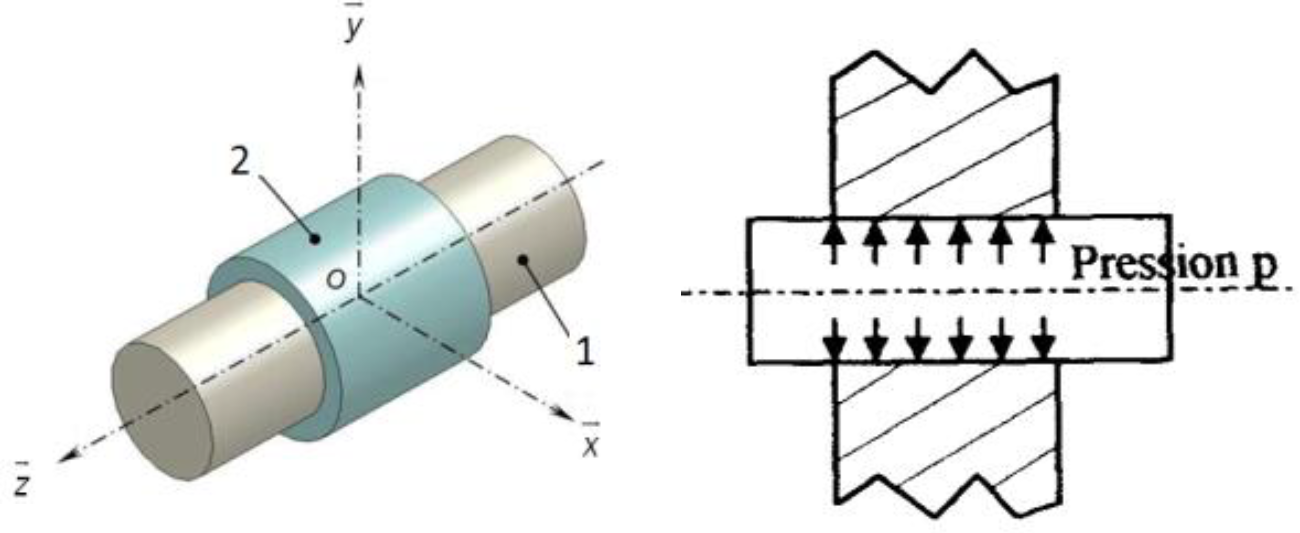
\includegraphics[width=\linewidth]{533_01}
\end{center}


\begin{obj}
Déterminer l’effort axial maximal transmissible et le couple maximal transmissible d’une pièce à 
l’autre.
\end{obj}




\subsection*{Couple maximal transmissible}


Le couple (ou moment) maximal transmissible correspond à la valeur maximale 
de la composante sur l’axe $\vect{z}$ du moment résultant de l’action mécanique qui peut 
être transmise d’une pièce à l’autre sans qu’elles se désolidarisent. 
 
Pour simplifier notre étude, on considère la pièce 2 fixe et on cherche à 
déterminer la composante sur l’axe $\vect{z}$ du moment résultant de l’action mécanique 
à appliquer à la pièce 1 pour atteindre le glissement de 1/2 autour de $\vect{z}$.
 

\begin{center}
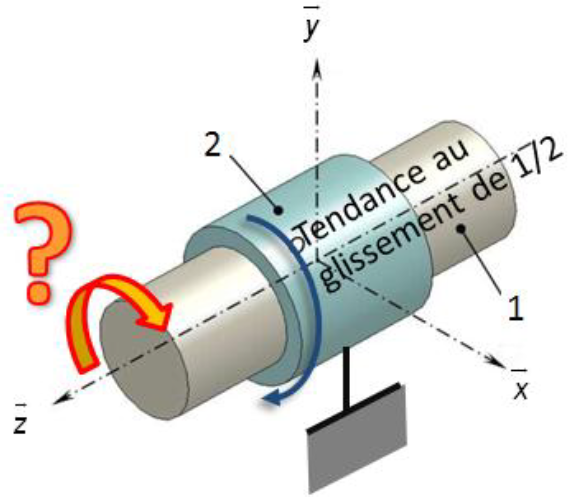
\includegraphics[width=.8\linewidth]{533_04}
\end{center}



\question{Refaire en grand les 2 schémas  : un 
dans le plan $(\vect{y}, \vect{z})$ et l’autre dans le plan $(\vect{x}, \vect{y})$, 
en plaçant les actions élémentaires normale et 
tangentielle de 2 sur 1 en un point $Q$ 
quelconque de la surface de contact. }


\begin{center}
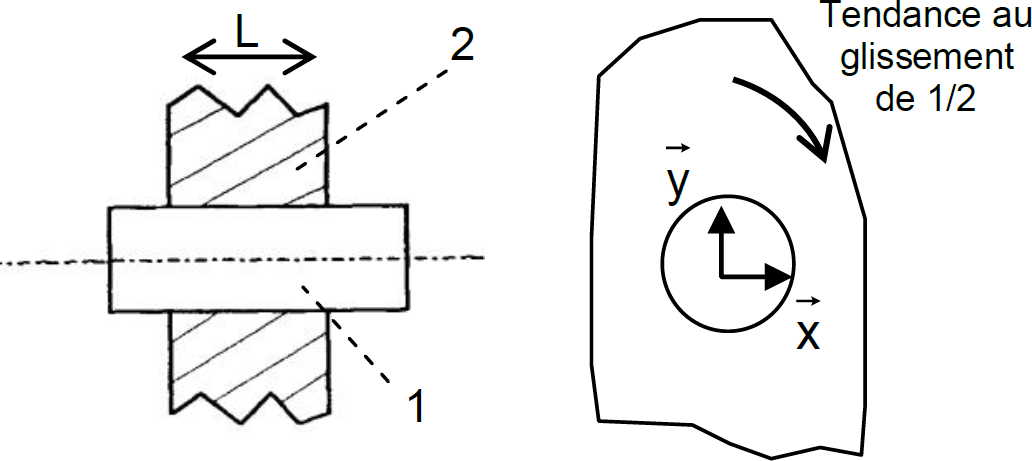
\includegraphics[width=.8\linewidth]{533_05}
\end{center}



\question{Exprimer $\vect{dF_{2\rightarrow 1}(Q)}$.}

\question{Déterminer le couple maximal transmissible en fonction de $p$ et des 
caractéristiques géométriques du frettage.}



\ifprof
\else
\begin{flushright}
\footnotesize{Corrigé  voir \ref{B2:14:Coulomb:533}.}
\end{flushright}%
\fi